% OpenResearch — system architecture
% Compile with:  pdflatex architecture.tex   (or: lualatex architecture.tex)
% Source of truth: CLAUDE.md (day-to-day tier-2 doc).
\documentclass[border=12pt]{standalone}

\usepackage{tikz}
\usepackage{newtxtext,newtxmath}
\usetikzlibrary{positioning,fit,backgrounds,arrows.meta,calc,shapes.geometric}

% ---------------------------------------------------------------------------
% Palette
% ---------------------------------------------------------------------------
\definecolor{cBand}{HTML}{F4F6FA}   % band background
\definecolor{cBandEdge}{HTML}{C2CCD9}
\definecolor{cUI}{HTML}{DCEBFB}     % frontend
\definecolor{cHTTP}{HTML}{D7E8DF}    % http / proxy
\definecolor{cRLM}{HTML}{E7DCF5}     % rlm engine
\definecolor{cRDR}{HTML}{FBE6CC}     % rdr engine
\definecolor{cPrim}{HTML}{F3E8FB}    % primitives
\definecolor{cSand}{HTML}{FAD9D9}    % sandbox
\definecolor{cAuth}{HTML}{FFF3C4}    % auth
\definecolor{cSSE}{HTML}{D5EFF0}     % sse
\definecolor{cStore}{HTML}{E3E6EB}   % persistence
\definecolor{cWarn}{HTML}{B3261E}    % warning text
\definecolor{cLine}{HTML}{5A6472}

% ---------------------------------------------------------------------------
% Styles
% ---------------------------------------------------------------------------
\tikzset{
  band/.style={
    draw=cBandEdge, fill=cBand, rounded corners=3pt, line width=0.8pt,
    inner sep=10pt},
  bandlabel/.style={
    font=\bfseries\footnotesize, text=cLine, anchor=north west},
  box/.style={
    draw=cBandEdge, rounded corners=2pt, line width=0.7pt,
    align=center, font=\scriptsize, inner sep=5pt, text width=30mm},
  wide/.style={box, text width=46mm},
  xwide/.style={box, text width=64mm},
  tag/.style={font=\scriptsize\bfseries},
  note/.style={font=\scriptsize\itshape, text=cLine, align=left},
  warn/.style={font=\scriptsize, text=cWarn, align=left},
  flow/.style={-{Stealth[length=2.4mm]}, line width=0.8pt, draw=cLine},
  flowd/.style={flow, dashed},
}

\begin{document}
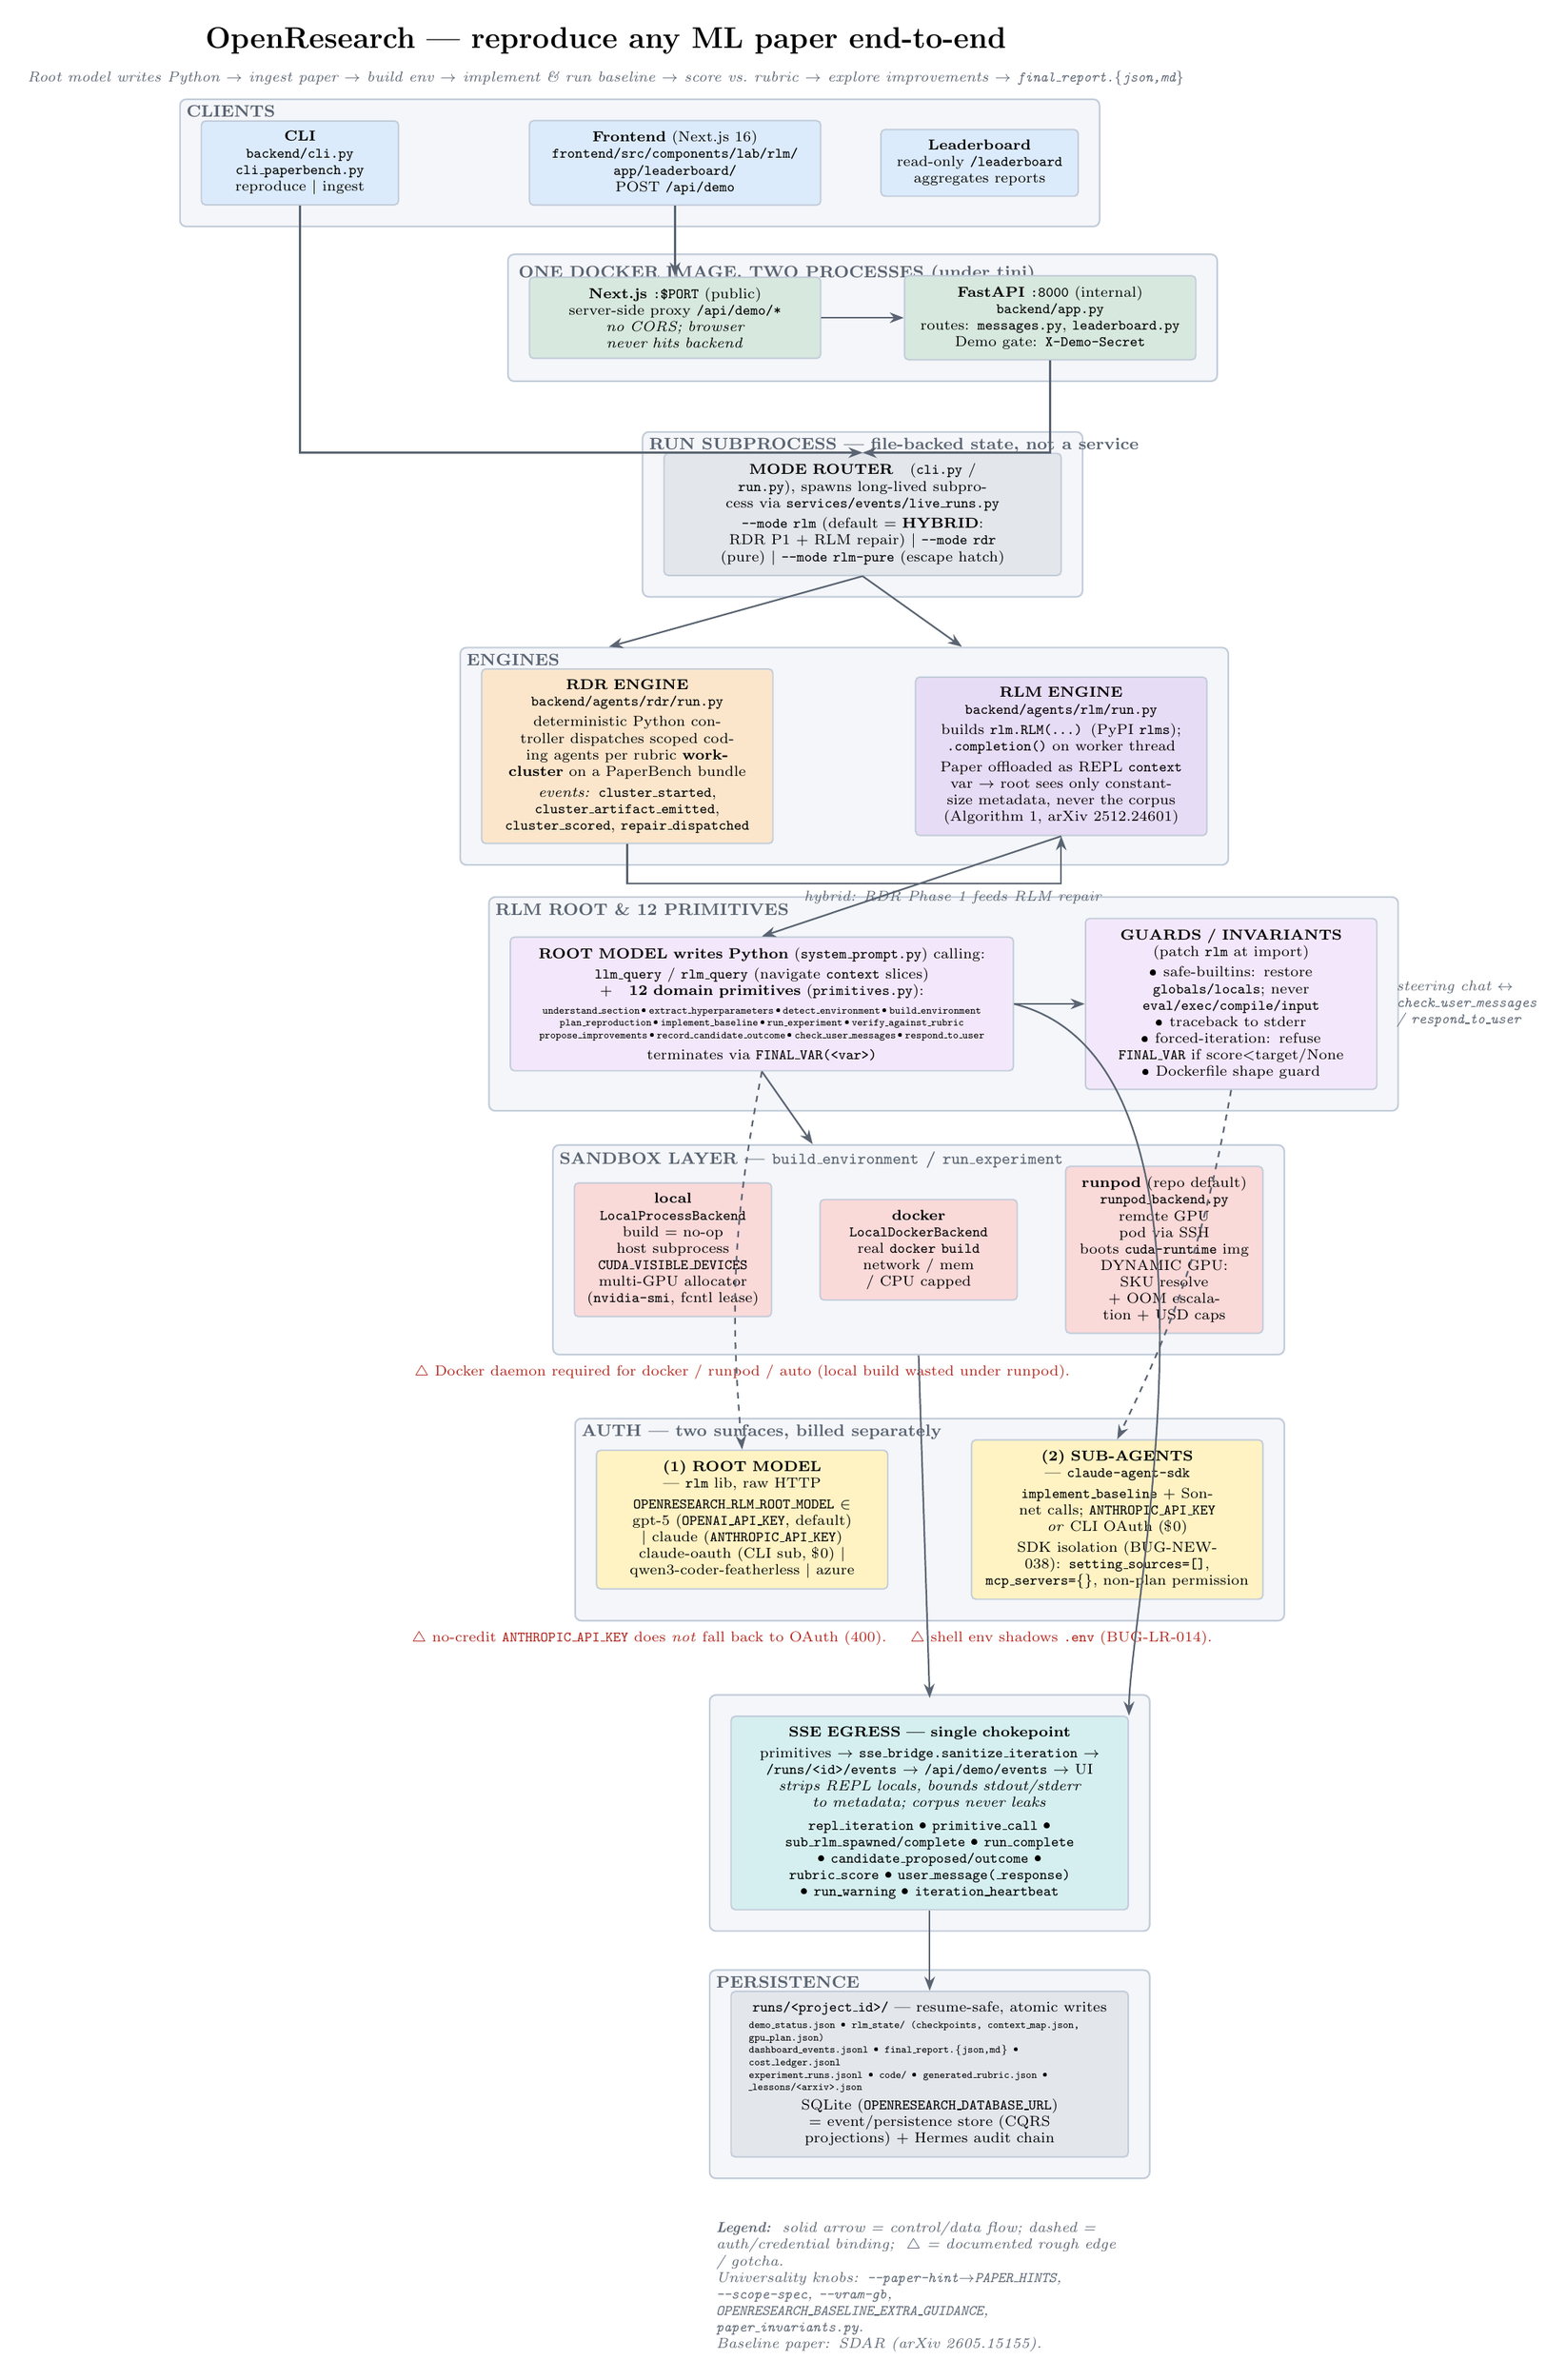
\begin{tikzpicture}[node distance=5mm]

% ===========================================================================
% TITLE
% ===========================================================================
\node[font=\Large\bfseries] (title)
  {OpenResearch --- reproduce any ML paper end-to-end};
\node[note, below=1pt of title]
  {Root model writes Python $\rightarrow$ ingest paper $\rightarrow$ build env
   $\rightarrow$ implement \& run baseline $\rightarrow$ score vs.\ rubric
   $\rightarrow$ explore improvements $\rightarrow$ \texttt{final\_report.\{json,md\}}};

% ===========================================================================
% BAND 1 — CLIENTS / ENTRY
% ===========================================================================
\node[box, fill=cUI, below=10mm of title.south, xshift=-52mm] (cli)
  {\textbf{CLI}\\\texttt{backend/cli.py}\\\texttt{cli\_paperbench.py}\\
   reproduce \textbar{} ingest};
\node[wide, fill=cUI, right=22mm of cli] (fe)
  {\textbf{Frontend} (Next.js 16)\\\texttt{frontend/src/components/lab/rlm/}\\
   \texttt{app/leaderboard/}\\POST \texttt{/api/demo}};
\node[box, fill=cUI, right=10mm of fe] (lb)
  {\textbf{Leaderboard}\\read-only \texttt{/leaderboard}\\aggregates reports};

\begin{scope}[on background layer]
  \node[band, fit=(cli)(fe)(lb)] (b1) {};
\end{scope}
\node[bandlabel] at (b1.north west) {CLIENTS};

% ===========================================================================
% BAND 2 — ONE IMAGE, TWO PROCESSES + HTTP
% ===========================================================================
\node[wide, fill=cHTTP, below=12mm of fe.south] (next)
  {\textbf{Next.js} \texttt{:\$PORT} (public)\\
   server-side proxy \texttt{/api/demo/*}\\\textit{no CORS; browser never hits backend}};
\node[wide, fill=cHTTP, right=14mm of next] (fast)
  {\textbf{FastAPI} \texttt{:8000} (internal)\\\texttt{backend/app.py}\\
   routes: \texttt{messages.py}, \texttt{leaderboard.py}\\
   Demo gate: \texttt{X-Demo-Secret}};

\begin{scope}[on background layer]
  \node[band, fit=(next)(fast),
        label={[bandlabel, anchor=north west, xshift=2pt, yshift=-2pt]north west:%
               ONE DOCKER IMAGE, TWO PROCESSES (under tini)}] (b2) {};
\end{scope}

% ===========================================================================
% BAND 3 — RUN SUBPROCESS: MODE ROUTER
% ===========================================================================
\node[xwide, fill=cStore, below=12mm of b2.south, anchor=north] (router)
  {\textbf{MODE ROUTER}\quad(\texttt{cli.py} / \texttt{run.py}),
   spawns long-lived subprocess via \texttt{services/events/live\_runs.py}\\[2pt]
   \texttt{--mode rlm} (default = \textbf{HYBRID}: RDR P1 + RLM repair)\ \textbar{}\
   \texttt{--mode rdr} (pure)\ \textbar{}\ \texttt{--mode rlm-pure} (escape hatch)};

\begin{scope}[on background layer]
  \node[band, fit=(router)] (b3) {};
\end{scope}
\node[bandlabel] at (b3.north west) {RUN SUBPROCESS — file-backed state, not a service};

% ===========================================================================
% BAND 4 — ENGINES
% ===========================================================================
\node[wide, fill=cRDR, below=12mm of b3.south, anchor=north, xshift=-40mm] (rdr)
  {\textbf{RDR ENGINE}\\\texttt{backend/agents/rdr/run.py}\\[2pt]
   deterministic Python controller dispatches scoped coding agents per rubric
   \textbf{work-cluster} on a PaperBench bundle\\[2pt]
   \textit{events:} \texttt{cluster\_started}, \texttt{cluster\_artifact\_emitted},
   \texttt{cluster\_scored}, \texttt{repair\_dispatched}};

\node[wide, fill=cRLM, right=24mm of rdr] (rlm)
  {\textbf{RLM ENGINE}\\\texttt{backend/agents/rlm/run.py}\\[2pt]
   builds \texttt{rlm.RLM(...)} (PyPI \texttt{rlms}); \texttt{.completion()} on worker thread\\[2pt]
   Paper offloaded as REPL \texttt{context} var $\rightarrow$ root sees only
   constant-size metadata, never the corpus (Algorithm~1, arXiv~2512.24601)};

\begin{scope}[on background layer]
  \node[band, fit=(rdr)(rlm)] (b4) {};
\end{scope}
\node[bandlabel] at (b4.north west) {ENGINES};

% ===========================================================================
% BAND 5 — RLM ROOT + 12 PRIMITIVES + GUARDS
% ===========================================================================
\node[xwide, text width=82mm, fill=cPrim, below=12mm of b4.south, anchor=north, xshift=-14mm] (prim)
  {\textbf{ROOT MODEL writes Python} (\texttt{system\_prompt.py}) calling:\\[2pt]
   \texttt{llm\_query} / \texttt{rlm\_query} (navigate \texttt{context} slices) \quad+\quad
   \textbf{12 domain primitives} (\texttt{primitives.py}):\\[3pt]
   \begin{minipage}{0.96\linewidth}\centering\ttfamily\tiny
   understand\_section\,\textbullet\,extract\_hyperparameters\,\textbullet\,detect\_environment\,\textbullet\,build\_environment\\
   plan\_reproduction\,\textbullet\,implement\_baseline\,\textbullet\,run\_experiment\,\textbullet\,verify\_against\_rubric\\
   propose\_improvements\,\textbullet\,record\_candidate\_outcome\,\textbullet\,check\_user\_messages\,\textbullet\,respond\_to\_user
   \end{minipage}\\[3pt]
   terminates via \texttt{FINAL\_VAR(<var>)}};

\node[wide, fill=cPrim, right=12mm of prim] (guards)
  {\textbf{GUARDS / INVARIANTS}\\(patch \texttt{rlm} at import)\\[2pt]
   \textbullet\ safe-builtins: restore \texttt{globals/locals};
   never \texttt{eval/exec/compile/input}\\
   \textbullet\ traceback to stderr\\
   \textbullet\ forced-iteration: refuse \texttt{FINAL\_VAR} if score$<$target/None\\
   \textbullet\ Dockerfile shape guard};

\begin{scope}[on background layer]
  \node[band, fit=(prim)(guards)] (b5) {};
\end{scope}
\node[bandlabel] at (b5.north west) {RLM ROOT \& 12 PRIMITIVES};

% steering loop note
\node[note, right=4mm of guards.east, text width=24mm, xshift=-2mm] (steer)
  {steering chat $\leftrightarrow$ \texttt{check\_user\_messages} / \texttt{respond\_to\_user}};

% ===========================================================================
% BAND 6 — SANDBOX
% ===========================================================================
\node[box, fill=cSand, below=12mm of b5.south, anchor=north, xshift=-46mm] (slocal)
  {\textbf{local}\\\texttt{LocalProcessBackend}\\build = no-op\\host subprocess\\
   \texttt{CUDA\_VISIBLE\_DEVICES}\\multi-GPU allocator\\(\texttt{nvidia-smi}, fcntl lease)};
\node[box, fill=cSand, right=8mm of slocal] (sdocker)
  {\textbf{docker}\\\texttt{LocalDockerBackend}\\real \texttt{docker build}\\
   network / mem / CPU capped};
\node[box, fill=cSand, right=8mm of sdocker] (srunpod)
  {\textbf{runpod} (repo default)\\\texttt{runpod\_backend.py}\\remote GPU pod via SSH\\
   boots \texttt{cuda-runtime} img\\DYNAMIC GPU: SKU resolve\\
   + OOM escalation + USD caps};

\begin{scope}[on background layer]
  \node[band, fit=(slocal)(sdocker)(srunpod)] (b6) {};
\end{scope}
\node[bandlabel] at (b6.north west)
  {SANDBOX LAYER — \texttt{build\_environment} / \texttt{run\_experiment}};
\node[warn, below=1pt of b6.south, xshift=-30mm]
  {$\triangle$ Docker daemon required for docker / runpod / auto (local build wasted under runpod).};

% ===========================================================================
% BAND 7 — AUTH (two surfaces)
% ===========================================================================
\node[wide, fill=cAuth, below=16mm of b6.south, anchor=north, xshift=-30mm] (auth1)
  {\textbf{(1) ROOT MODEL} — \texttt{rlm} lib, raw HTTP\\[2pt]
   \texttt{OPENRESEARCH\_RLM\_ROOT\_MODEL} $\in$\\
   gpt-5 (\texttt{OPENAI\_API\_KEY}, default) \textbar{} claude (\texttt{ANTHROPIC\_API\_KEY})\\
   claude-oauth (CLI sub, \$0) \textbar{} qwen3-coder-featherless \textbar{} azure};
\node[wide, fill=cAuth, right=14mm of auth1] (auth2)
  {\textbf{(2) SUB-AGENTS} — \texttt{claude-agent-sdk}\\[2pt]
   \texttt{implement\_baseline} + Sonnet calls;
   \texttt{ANTHROPIC\_API\_KEY} \emph{or} CLI OAuth (\$0)\\[2pt]
   SDK isolation (BUG-NEW-038): \texttt{setting\_sources=[]},
   \texttt{mcp\_servers=\{\}}, non-plan permission};

\begin{scope}[on background layer]
  \node[band, fit=(auth1)(auth2)] (b7) {};
\end{scope}
\node[bandlabel] at (b7.north west) {AUTH — two surfaces, billed separately};
\node[warn, below=1pt of b7.south, xshift=-20mm]
  {$\triangle$ no-credit \texttt{ANTHROPIC\_API\_KEY} does \emph{not} fall back to OAuth
   (400). \quad $\triangle$ shell env shadows \texttt{.env} (BUG-LR-014).};

% ===========================================================================
% BAND 8 — SSE EGRESS
% ===========================================================================
\node[xwide, fill=cSSE, below=16mm of b7.south, anchor=north] (sse)
  {\textbf{SSE EGRESS — single chokepoint}\\[2pt]
   primitives $\rightarrow$ \texttt{sse\_bridge.sanitize\_iteration} $\rightarrow$
   \texttt{/runs/<id>/events} $\rightarrow$ \texttt{/api/demo/events} $\rightarrow$ UI\\
   \textit{strips REPL locals, bounds stdout/stderr to metadata; corpus never leaks}\\[3pt]
   \scriptsize\ttfamily repl\_iteration \textbullet\ primitive\_call \textbullet\ sub\_rlm\_spawned/complete
   \textbullet\ run\_complete \textbullet\ candidate\_proposed/outcome \textbullet\ rubric\_score
   \textbullet\ user\_message(\_response) \textbullet\ run\_warning \textbullet\ iteration\_heartbeat};

\begin{scope}[on background layer]
  \node[band, fit=(sse)] (b8) {};
\end{scope}

% ===========================================================================
% BAND 9 — PERSISTENCE
% ===========================================================================
\node[xwide, fill=cStore, below=10mm of b8.south, anchor=north] (store)
  {\texttt{runs/<project\_id>/} — resume-safe, atomic writes\\[2pt]
   \begin{minipage}{0.96\linewidth}\tiny\ttfamily
   demo\_status.json \textbullet\ rlm\_state/ (checkpoints, context\_map.json, gpu\_plan.json)\\
   dashboard\_events.jsonl \textbullet\ final\_report.\{json,md\} \textbullet\ cost\_ledger.jsonl\\
   experiment\_runs.jsonl \textbullet\ code/ \textbullet\ generated\_rubric.json \textbullet\ \_lessons/<arxiv>.json
   \end{minipage}\\[2pt]
   \textnormal{\scriptsize SQLite (\texttt{OPENRESEARCH\_DATABASE\_URL}) = event/persistence store (CQRS projections) + Hermes audit chain}};

\begin{scope}[on background layer]
  \node[band, fit=(store)] (b9) {};
\end{scope}
\node[bandlabel] at (b9.north west) {PERSISTENCE};

% ===========================================================================
% FLOWS (vertical spine + key cross-links)
% ===========================================================================
\draw[flow] (cli.south) |- (router.north);
\draw[flow] (fe.south) -- (next.north);
\draw[flow] (next.east) -- (fast.west);
\draw[flow] (fast.south) |- (router.north);

\draw[flow] (router.south) -- ([xshift=-40mm]b4.north);  % to rdr
\draw[flow] (router.south) -- ([xshift=20mm]b4.north);    % to rlm
\draw[flow] (rdr.south) |- ($(b4.south)+(0,-3mm)$) -| (rlm.south)
  node[note, pos=0.25, below]{hybrid: RDR Phase~1 feeds RLM repair};

\draw[flow] (rlm.south) -- (prim.north);
\draw[flow] (prim.south) -- ([xshift=-18mm]b6.north);     % primitives -> sandbox
\draw[flow] (prim.east) -- (guards.west);

\draw[flowd] (prim.south) to[bend right=8] (auth1.north);  % root auth
\draw[flowd] (guards.south) to[bend left=8] (auth2.north); % sub-agent auth

\draw[flow] (b6.south) -- ([yshift=3mm]sse.north);
\draw[flow] (prim.east) .. controls +(40mm,-10mm) and +(0,18mm) .. (sse.north east);
\draw[flow] (sse.south) -- (store.north);

% legend ---------------------------------------------------------------------
\node[note, anchor=north west, text width=70mm] at ([yshift=-6mm]b9.south west)
  {\textbf{Legend:}\ \ solid arrow = control/data flow;\ dashed = auth/credential
   binding;\ \ $\triangle$ = documented rough edge / gotcha.\\
   Universality knobs: \texttt{--paper-hint}$\rightarrow$\texttt{PAPER\_HINTS},
   \texttt{--scope-spec}, \texttt{--vram-gb},
   \texttt{OPENRESEARCH\_BASELINE\_EXTRA\_GUIDANCE}, \texttt{paper\_invariants.py}.\\
   Baseline paper: SDAR (arXiv~2605.15155).};

\end{tikzpicture}
\end{document}
